%%%%%%%%%%%%%%%%%%%%%%%%%%%%%%%%%%%%%%%%%%%%%%%%%%%%%%%%%%%%%%%%%%%%%%%%%%
%%%%%                         CHAPITRE 7                            %%%%%%
%%%%%%%%%%%%%%%%%%%%%%%%%%%%%%%%%%%%%%%%%%%%%%%%%%%%%%%%%%%%%%%%%%%%%%%%%%

\lhead[\fancyplain{}{\leftmark}]%Pour les pages paires \bfseries
      {\fancyplain{}{}} %Pour les pages impaires
\chead[\fancyplain{}{}]%
      {\fancyplain{}{}}
\rhead[\fancyplain{}{}]%Pour les pages paires 
      {\fancyplain{}{\rightmark}}%Pour les pages impaires \bfseries
\lfoot[\fancyplain{}{}]%
      {\fancyplain{}{}}
\cfoot[\fancyplain{}{\thepage}]%\bfseries
      {\fancyplain{}{\thepage}} %\bfseries
\rfoot[\fancyplain{}{}]%
     {\fancyplain{}{\scriptsize}}


%%%%%%%%%%%%%%%%%%%%%%%%%%%%%%%%%%%%%%%%%%%%%%%%%%%%%%%%%%%%%%%%%%%%%%%%%%
%%%%%                      Start part here                          %%%%%%
%%%%%%%%%%%%%%%%%%%%%%%%%%%%%%%%%%%%%%%%%%%%%%%%%%%%%%%%%%%%%%%%%%%%%%%%%%

\chapter{Application to BMX racing, jointly capturing pilot and bike}
\label{ch:7}

%==============================================================================	Résumé du chapitre

\begin{center}
\rule{0.7\linewidth}{.5pt}
\begin{minipage}{0.7\linewidth}
\smallskip

\textit{Numerous sports disciplines are practiced with special equipment, such as a board in skateboarding, a racket and a ball in tennis, or a bike in BMX racing. The interactions between the athlete and their gear are often important to retrieve. We analyzed a BMX start sequence, by using OpenPose for 2D human pose estimation, and a custom trained DeepLabCut model for bike detection. We ran Pose2Sim on the joint {pilot+bike} 2D estimations, and performed 3D inverse kinematics on a custom OpenSim {pilot+bike} model. This showed that analyzing simultaneously the athlete and their equipment is possible, which provides additional perspectives for markerless sports motion analysis.\newline
See Figure~\ref{fig_visabstract5} for a visual abstract.
}

%\smallskip
\end{minipage}
\smallskip
\rule{0.7\linewidth}{.5pt}
\end{center}

\newpage

\minitoc

\vspace*{3cm}

\begin{figure}[hbtp]
	\centering
	\def\svgwidth{1\columnwidth}
	\fontsize{10pt}{10pt}\selectfont
	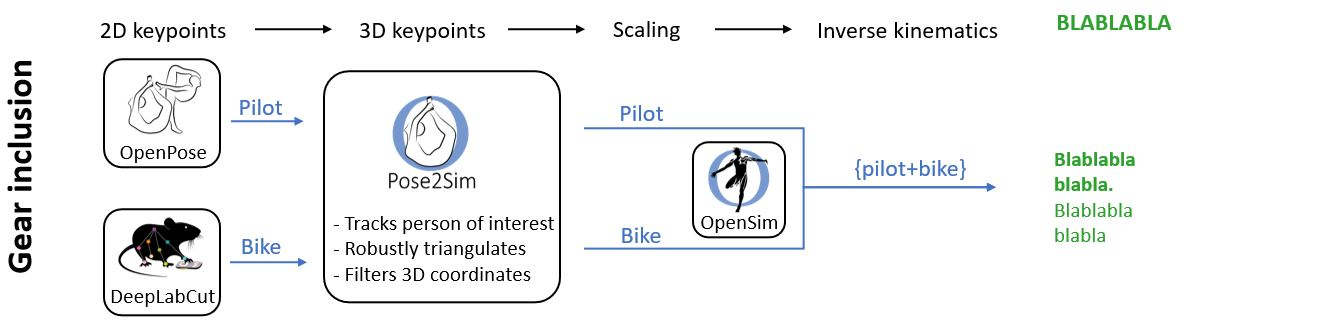
\includegraphics[width=\linewidth]{"../Intro/Figures/Fig_VisAbstract5.JPG"}
      \caption{Visual abstract for joint analysis of the athlete with OpenPose, and their equipment with DeepLabCut.}
	\label{fig_visabstract5}
\end{figure}

\newpage


Ski: lire intro sur equipement: https://sci-hub.se/https://ieeexplore.ieee.org/document/9105973 
Formalisme joint vs constraint Part 3.1 https://sci-hub.se/https://ieeexplore.ieee.org/document/4587520
https://www.google.com/search?client=firefox-b-e&q=constraint+vs+joint
https://arxiv.org/pdf/2112.00627.pdf 42: ball as segmentation. eux: keypoint




Preliminary experiment


1. track equipment (shape or keypoints), Straight-forward with markers (hockey kays2017) or IMUs (boat ruffaldi2015), whereas specific training for markerless deep-learning (bike-snow Rosenhahn2008, ball Ghasemzadeh2021, skis ludwig2020)
2. compute joint kinematics of the equipment (6DoF, or definition of model with kinematic chain) 
3. solve combined kinematics of the whole system (closed loop)

Chap3:
On a different note, in a sports context, not only the human pose is of interest: sports gear can also be considerably important to detect, such as a ball \cite{Ghasemzadeh2021}, a hockey stick \cite{Kays2017}, a rowing boat\cite{Ruffaldi2015}, a snowboard \cite{Rosenhahn2008} or skis \cite{Ludwig2020}, or bike parts in the context of cycling (see Chapter 7 on \hyperref[ch:7]{Joint OpenPose and DeepLabCut detection}). This can help to analyze game dynamics, and to quantify posture cues related to a specific sports discipline. This can be done, for example, by separately process the video with OpenPose, as well as with a custom-trained DeepLabCut model. Resulting .trc coordinate files can be merged, and used in OpenSim. However, the DeeLabCut keypoints must be referenced on an OpenSim model, which may need to be crafted from scratch, such as a ball, skis, or bike, depending on the detected object.


CF mail OpenPose DeepLabCut pour BMX
pre manip, slt 6 cam, calib unsuccessful: on grid similar to other chapter, low image resolution
other leads: bushing forces, ball joints
scale avant et arriève vélo indépendament
% Because OpenSim models have fewer degrees of freedom than the human body, it is easy to define a set of constraints that seems very reasonable but is not easy for the skeleton (rigid-body mechanism) to satisfy.
% If it's appropriate for the movement you are simulating, you might consider allowing the toes and/or hands to rotate relative to the pedals
% (see PointConstraint, https://simtk.org/api_docs/opensim/api_docs/classOpenSim_1_1PointConstraint.html#details).
% Alternatively, you could attach the toes and/or hands to the bike via BushingForces (https://simtk.org/api_docs/opensim/api_docs/classOpenSim_1_1BushingForce.html#details).


\section{Introduction}
\subsection{The importance of equipment}


\subsection{The start in BMX racing}



\section{Methods}
\subsection{Material and protocol}


\subsection{Pilot inverse kinematics}


\subsection{Bike inverse kinematics}

Voir thèse Princelle


\subsection{Joined pilot and bike inverse kinematics}
Marche pas avec nos qualités de vidéo : simulations



\begin{figure}[hbtp]
	\centering
	\def\svgwidth{1\columnwidth}
	\fontsize{10pt}{10pt}\selectfont
	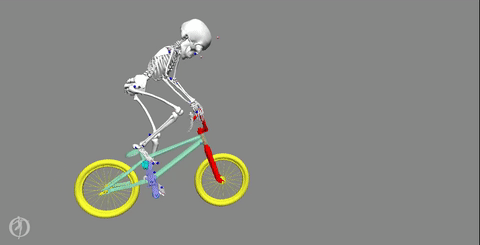
\includegraphics[width=\linewidth]{"../Chap7/Figures/BMXPilot.png"}
	\caption{Note that the head is only big because the pilot was scaled with his helmet on. Since the head is at the end of the kinematic chain, and as kinetics are not addressed, it does not affect inverse kinematics. See animated version \href{https://github.com/perfanalytics/pose2sim/blob/main/Content/Activities_verylow.gif}{here}.}
	\label{fig_bmxpilot}
\end{figure}

% \begin{frame}{Embedded Animation}
%   \animategraphics[loop,controls,width=0.7\linewidth]{25}{"../Chap7/Figures/bmxgif/bmx"}{1}{180}
% \end{frame}



\section{Results}



\section{Discussion}
\subsection{On these data}


\subsection{Limits and perspectives}


Rosenhahn2008 snowboard: closed kinematic chain: pas évident, voir [17] ( reduced equations of robotic systems using Lie groups). Eux: soft constraints (invariances -> numeric) rather than joints (analytic)

Mathis2020 Principles, pitfalls and perspectives

% ajouter video de use on your own data
splashes, occlusions, distance, etc

Voir Protocole doc: % https://1drv.ms/w/s!AvGG4T_aAnWzmy4JuQph05pIphXX?e=0yjqbs
